\documentclass[a4paper]{report}
% Some basic packages
\usepackage[utf8]{inputenc}
\usepackage[T1]{fontenc}
\usepackage{textcomp}
\usepackage{url}
\usepackage{graphicx}
\usepackage{float}
\usepackage{booktabs}
\usepackage{enumitem}
\usepackage[hidelinks, urlcolor=blue]{hyperref}

\pdfminorversion=7

% Don't indent paragraphs, leave some space between them
\usepackage{parskip}

% for the big braces
\usepackage{bigdelim}

% Hide page number when page is empty
\usepackage{emptypage}
\usepackage{subcaption}
\usepackage{multicol}
\usepackage{xcolor}

% Math stuff
\usepackage{amsmath, amsfonts, mathtools, amsthm, amssymb}
% Fancy script capitals
\usepackage{mathrsfs}
\usepackage{cancel}
% Bold math
\usepackage{bm}

% Add \contd symbol to denote contradiction
\usepackage{stmaryrd} % for \lightning
\newcommand\contd{\scalebox{1.5}{$\lightning$}}

% \let\phi\varphi

% Command for short corrections
% Usage: 1+1=\correct{3}{2}

\definecolor{correct}{HTML}{009900}
\newcommand\correct[2]{\ensuremath{\:}{\color{red}{#1}}\ensuremath{\to }{\color{correct}{#2}}\ensuremath{\:}}
\newcommand\green[1]{{\color{correct}{#1}}}

% horizontal rule
\newcommand\hr{
	\noindent\rule[0.5ex]{\linewidth}{0.5pt}
}

% hide parts
\newcommand\hide[1]{}

% si unix
\usepackage{siunitx}

% Environments
\makeatother
% For box around Definition, Theorem, \ldots
\usepackage{mdframed}
\mdfsetup{skipabove=1em,skipbelow=0em}
\theoremstyle{definition}
\newmdtheoremenv[nobreak=true]{definition}{Definition}
\newtheorem*{eg}{Example}
\newtheorem*{notation}{Notation}
\newtheorem*{prev}{As previously seen}
\newtheorem*{remark}{Remark}
\newtheorem*{note}{Note}
\newtheorem*{problem}{Problem}
\newtheorem*{answer}{Answer}
\newtheorem*{observe}{Observe}
\newtheorem*{property}{Property}
\newtheorem*{intuition}{Intuition}
\newmdtheoremenv[nobreak=true]{prop}{Proposition}
\newmdtheoremenv[nobreak=true]{lemma}{Lemma}
\newmdtheoremenv[nobreak=true]{theorem}{Theorem}
\newmdtheoremenv[nobreak=true]{corollary}{Corollary}

% Fix some spacing
% http://tex.stackexchange.com/questions/22119/how-can-i-change-the-spacing-before-theorems-with-amsthm
\makeatletter
\def\thm@space@setup{%
	\thm@preskip=\parskip \thm@postskip=0pt
}

\usepackage{xifthen}
\def\testdateparts#1{\dateparts#1\relax}
\def\dateparts#1 #2 #3 #4 #5\relax{
	\marginpar{\small\textsf{\mbox{#1 #2 #3 #5}}}
}

\def\@lecture{}%
\newcommand{\lecture}[3]{
	\ifthenelse{\isempty{#3}}{%
		\def\@lecture{Lecture #1}%
	}{%
		\def\@lecture{Lecture #1: #3}%
	}%
	\subsection*{\@lecture}
	\marginpar{\small\textsf{\mbox{#2}}}
}

% These are the fancy headers
\usepackage{fancyhdr}
\pagestyle{fancy}

% LE: left even
% RO: right odd
% CE, CO: center even, center odd
% My name for when I print my lecture notes to use for an open book exam.
% \fancyhead[LE,RO]{Gilles Castel}

\fancyhead[RO,LE]{\@lecture} % Right odd,  Left even
\fancyhead[RE,LO]{}          % Right even, Left odd

\fancyfoot[RO,LE]{\thepage}  % Right odd,  Left even
\fancyfoot[RE,LO]{}          % Right even, Left odd
\fancyfoot[C]{\leftmark}     % Center

\makeatother

% TodoNotes and inline notes in fancy boxes
\usepackage{todonotes}
\usepackage{tcolorbox}

% Make boxes breakable
\tcbuselibrary{breakable}

% Figure support as explained in my blog post.
\usepackage{import}
\usepackage{xifthen}
\usepackage{pdfpages}
\usepackage{transparent}
\newcommand{\incfig}[1]{%
	\def\svgwidth{\columnwidth}
	\import{./figures/}{#1.pdf_tex}
}

% useful macro for class
\newcommand{\probability}[1]{\mathbb{\MakeUppercase{P}}\left( #1 \right)}
\newcommand{\variance}[1]{\mathrm{Var}\left[ #1 \right]}
\newcommand{\expectation}[1]{\mathbb{\MakeUppercase{E}}\left[ #1 \right]}
\newcommand{\at}[3]{\left.#1\right\vert_{#2}^{#3}}

% Fix some stuff
% %http://tex.stackexchange.com/questions/76273/multiple-pdfs-with-page-group-included-in-a-single-page-warning
\pdfsuppresswarningpagegroup=1

\renewcommand{\qed}{\hfill$\blacksquare$}

\newcommand*{\MaxNumOfChapters}{10}% Adjust these two settings for your needs.
\newcommand*{\MaxNumOfSections}{6}%

\usepackage{pgffor}%

\newcommand{\lec}[2]{%
	\foreach \c in {#1,...,#2}{%
			\IfFileExists{Lectures/lec_\c.tex} {%
				\input{Lectures/lec_\c.tex}%
			}{}%
		}%
}
\author{Pingbang Hu}
\title{MATH635\\Riemannian Geometry}

\thispagestyle{empty}
\addbibresource{ref.bib}

\setlength\multicolsep{0pt}

\DeclareMathOperator{\Ind}{Ind}

\begin{document}

\maketitle

\begin{abstract}
	This is the advanced graduate-level differential geometry course focused on Riemannian geometry taught by \href{http://www-personal.umich.edu/~lbieri/}{Lydia Bieri}. Topics include local and global aspects of differential geometry and the relation with the underlying topology. We'll use do Carmo's \emph{Riemannian Geometry}~\cite{flaherty2013riemannian} as our reference; while not required, but highly recommended have on. Apart from this, I also found~\cite{Frederic2015} very useful.

	A noticeable different is that we introduce \hyperref[def:geodesic]{geodesics} differently from do Carmo~\cite{flaherty2013riemannian}, where we set the solution of the variations of \hyperref[def:energy]{energy} to define a \hyperref[def:geodesic]{geodesic} first, and then draw connection to the ``\hyperref[def:curve]{curve} with zero acceleration'' after introduce the \hyperref[def:covariant-derivative]{covariant derivative}; however, do Carmo~\cite{flaherty2013riemannian} first introduce \hyperref[def:covariant-derivative]{covariant derivative} and then return the variation view point much later.

	\vfill
	\begin{center}
		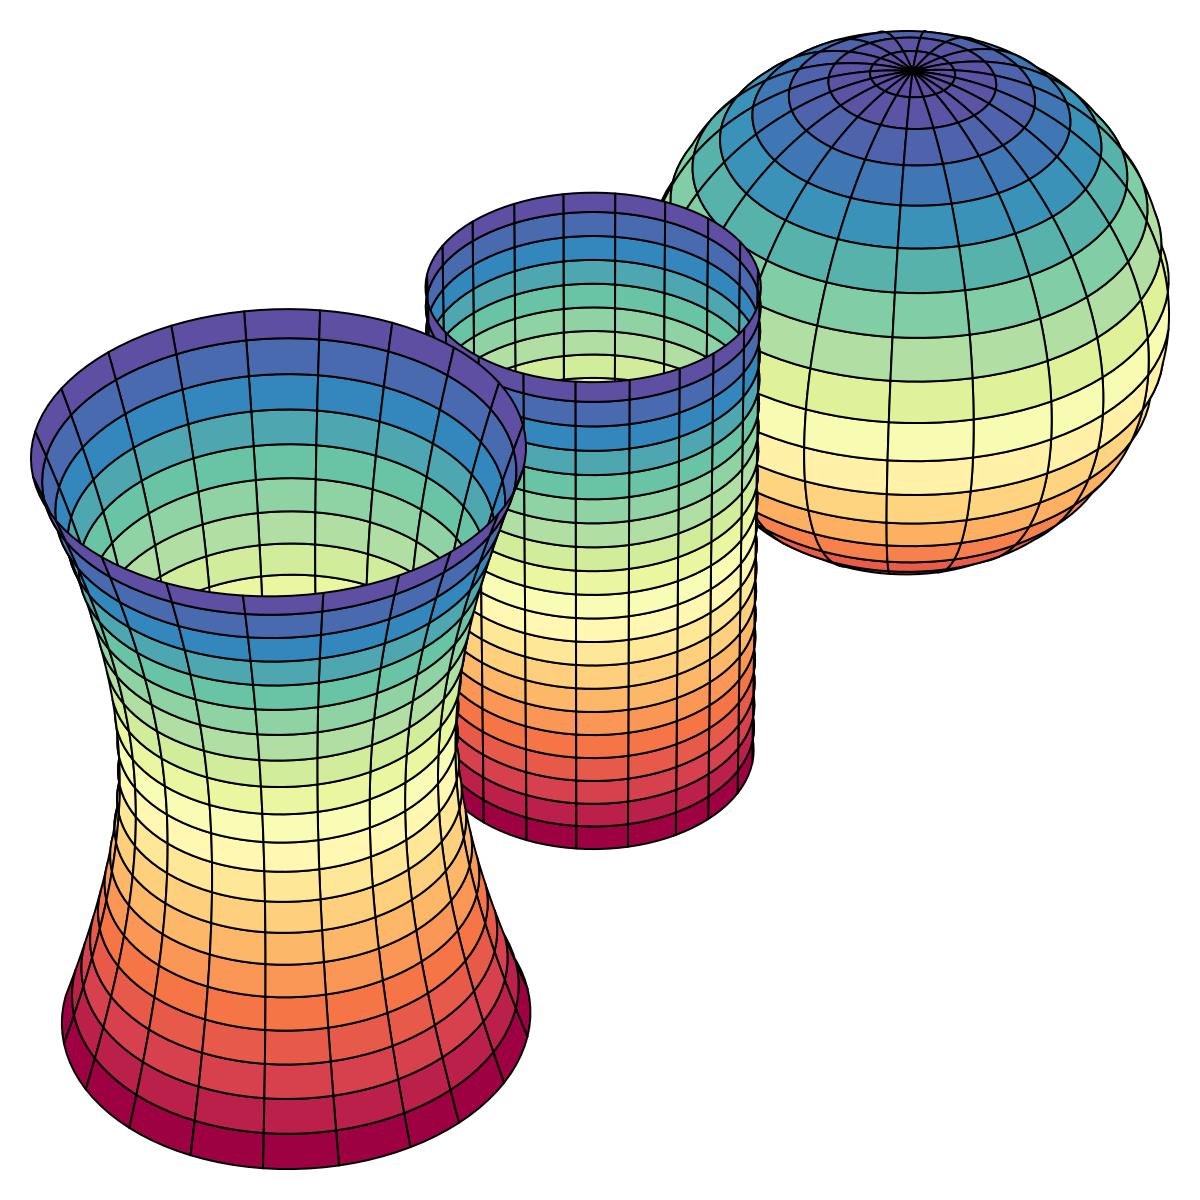
\includegraphics[width=.8\linewidth]{Figures/cover.png}
	\end{center}
	\vfill
	This course is taken in Winter 2023, and the date on the covering page is the last updated time.
\end{abstract}

\tableofcontents

\lec{1}{25}

\newpage
%─────Appendix────────────────────────────────────────────────────────────────────────────────────────────────────────────────────────────────────────
\appendix
\appendixpage

\chapter{Lie Groups and Lie Algebra}\label{ch:Lie-group-and-Lie-algebra}
\section{Lie Groups}
\hyperref[def:Lie-group]{Lie groups} are an important topic to study for Riemannian geometry, hence we now introduce it now.

\begin{definition}[Lie group]\label{def:Lie-group}
	A \emph{Lie group} is a group \(G\) with a \hyperref[def:smooth-structure]{differentiable structure} such that the mapping \(G \times G \to G\) given by \((x, y) \to xy^{-1} \), \(x, y\in G\), is differentiable.
\end{definition}

\begin{definition*}[Transformation]
	Let \(G\) be a \hyperref[def:Lie-group]{Lie group}.
	\begin{definition}[Left transformation]\label{def:left-transformation}
		The \emph{translations from the left} \(L_x \colon G \to G\) is defined as \(L_x(y) = xy\).
	\end{definition}
	\begin{definition}[Right transformation]\label{def:right-transformation}
		The \emph{translations from the right} \(R_x \colon G \to G\) is defined as \(R_x(y) = yx\).
	\end{definition}
\end{definition*}

\begin{remark}
	Both \(L_x\) and \(R_x\) are \hyperref[def:diffeomorphism]{diffeomorphisms}.
\end{remark}

In the following discussion, let \(G\) be a \hyperref[def:Lie-group]{Lie group}. Turns out that \(G\) admits some nice properties on \hyperref[def:vector-field-left-invariant]{left invariant} \hyperref[def:vector-field]{vector fields}.

\begin{definition*}[Invariant of Riemannian metric]
	Let \(g\) be a \hyperref[def:Riemannian-metric]{Riemannian metric} on \(G\).

	\begin{definition}[Left invariant]\label{def:Riemannian-metric-left-invariant}
		\(g\) is \emph{left invariant} if
		\[
			\left\langle u, v \right\rangle _y = \left\langle \mathrm{d} (L_x)_y u, \mathrm{d} (L_x)_y v \right\rangle _{L_x(y)}
		\]
		for all \(x, y\in G\), \(u, v\in T_y G\), i.e., \(L_x\) is an \hyperref[def:isometry]{isometry}.
	\end{definition}

	\begin{definition}[Right invariant]\label{def:Riemannian-metric-right-invariant}
		\(g\) is \emph{right invariant} if
		\[
			\left\langle u, v \right\rangle _y = \left\langle \mathrm{d} (R_x)_y u, \mathrm{d} (R_x)_y v \right\rangle _{R_x(y)}
		\]
		for all \(x, y\in G\), \(u, v\in T_y G\), i.e., \(R_x\) is an \hyperref[def:isometry]{isometry}.
	\end{definition}

	\begin{definition}[Bi-invariant]\label{def:Riemannian-metric-bi-invariant}
		\(g\) is \emph{bi-invariant} if it's both \hyperref[def:Riemannian-metric-right-invariant]{right} and \hyperref[def:Riemannian-metric-left-invariant]{left invariant}.
	\end{definition}
\end{definition*}

\begin{definition*}[Invariant of vector field]
	Let \(X\) be a \hyperref[def:vector-field]{vector field} on \(G\).

	\begin{definition}[Left invariant]\label{def:vector-field-left-invariant}
		\(X\) is \emph{left invariant} if \(\mathrm{d} L_x X = X\) for all \(x\in G\).
	\end{definition}

	\begin{definition}[Right invariant]\label{def:vector-field-right-invariant}
		\(X\) is \emph{right invariant} if \(\mathrm{d} R_x X = X\) for all \(x\in G\).
	\end{definition}

	\begin{definition}[Bi-invariant]\label{def:vector-field-bi-invariant}
		\(X\) is \emph{bi-invariant} if it's both \hyperref[def:vector-field-right-invariant]{right} and \hyperref[def:vector-field-left-invariant]{left invariant}.
	\end{definition}
\end{definition*}

As we mentioned, the \hyperref[def:vector-field-left-invariant]{left invariant} \hyperref[def:vector-field]{vector fields} are completely determined by their values at a single point of \(G\), which allows us to introduce an additional structure on the \hyperref[def:tangent-space]{tangent space} to the neutral element \(e\in G\) in the following manner.

To each \hyperref[def:tangent-vector]{vector} \(X_e\in T_e G\), we associate the \hyperref[def:vector-field-left-invariant]{left invariant} \(X\) defined by
\[
	X_a \coloneqq \mathrm{d} L_a X_e,\quad a\in G.
\]

\section{Lie Algebras}
Let \(X, Y\) be \hyperref[def:vector-field-left-invariant]{left invariant} \hyperref[def:vector-field]{vector fields} on \(G\). Since for each \(x\in G\) and for any differentiable function \(f\) on \(G\),
\[
	\mathrm{d} L_x [X, Y] f = [X, Y](f \circ L_x) = X(\mathrm{d} L_x Y) f - Y(\mathrm{d} L_x X) f = (XY - YX) f = [X, Y]f,
\]
i.e., \([X, Y]\) is again a \hyperref[def:vector-field-left-invariant]{left invariant} \hyperref[def:vector-field]{vector field} if \(X, Y\) are. Now, if \(X_e, Y_e\in T_e G\), we put \([X_e, Y_e] = [X, Y]_e\).

\begin{definition}[Lie algebra]\label{def:Lie-algebra}
	The \emph{Lie algebra} of \(G\), denoted by \(\mathfrak{g}\), is the vector space \(T_e G\) with the \hyperref[def:bracket]{bracket} \([\cdot, \cdot]\).
\end{definition}

\begin{note}
	The elements in the \hyperref[def:Lie-algebra]{Lie algebra} \(\mathfrak{g}\) will be thought of either as \hyperref[def:tangent-vector]{vectors} in \(T_e G\) or as \hyperref[def:vector-field-left-invariant]{left invariant} \hyperref[def:vector-field]{vector fields} on \(G\).
\end{note}

To introduce a \hyperref[def:Riemannian-metric-left-invariant]{left invariant} \hyperref[def:Riemannian-metric]{metric} on \(g\), take any arbitrary inner product \(\left\langle \cdot, \cdot \right\rangle _e\) on \(\mathfrak{g} \) and define
\begin{equation}\label{eq:inner-product-on-Lie-algebra}
	\left\langle u, v \right\rangle _x \coloneqq \left\langle (\mathrm{d} L_{x ^{-1} })_x(u), (\mathrm{d} L_{x ^{-1} })_x(v) \right\rangle _e
\end{equation}
for \(x\in G\), \(u, v\in T_x G\). Since \(L_x\) depends differentiably on \(x\), this is actually a \hyperref[def:Riemannian-metric]{Riemannian metric}, which is clearly \hyperref[def:Riemannian-metric-left-invariant]{left invariant}.

\begin{remark}
	We can also construct a \hyperref[def:Riemannian-metric-right-invariant]{right invariant} \hyperref[def:Riemannian-metric]{metric} on \(G\), and if \(G\) is compact, \(G\) possesses a \hyperref[def:Riemannian-metric-left-invariant]{bi-invariant} \hyperref[def:Riemannian-metric]{metric}.
\end{remark}

One important characterization for \(G\) having a \hyperref[def:Riemannian-metric-left-invariant]{bi-invariant} \hyperref[def:Riemannian-metric]{metric} is that the inner product that the \hyperref[def:Riemannian-metric]{metric} determines on \(\mathfrak{g} \) satisfies the following relation.

\begin{proposition}
	If \(G\) has a \hyperref[def:Riemannian-metric-left-invariant]{bi-invariant} \hyperref[def:Riemannian-metric]{metric}, then for any \(U, V, X\in \mathfrak{g} \), the inner product that the \hyperref[def:Riemannian-metric]{metric} determines on \(\mathfrak{g} \) satisfies
	\[
		\left\langle [U, X], V \right\rangle = -\left\langle U, [V, X] \right\rangle.
	\]
\end{proposition}
\begin{proof}
	See do Carmo~\cite[Page 40, 41]{flaherty2013riemannian}.
\end{proof}

The important point about this relation is that it characterizes the \hyperref[def:Riemannian-metric-left-invariant]{bi-invariant} \hyperref[def:Riemannian-metric]{metrics} of \(G\) in the following sense.

\begin{remark}
	If a positive bilinear form \(\left\langle \cdot, \cdot \right\rangle _e \) defined on \(\mathfrak{g} \) satisfies this relation, then the \hyperref[def:Riemannian-metric]{Riemannian metrics} defined on \(G\) by \autoref{eq:inner-product-on-Lie-algebra} is \hyperref[def:Riemannian-metric-left-invariant]{bi-invariant}.
\end{remark}

\newpage
%─────Reference──────────────────────────────────────────────────────────────────────────────────────────────────────────────────────────────────────
\printbibliography

\end{document}